\documentclass[12pt]{beamer}
\usepackage[T1]{fontenc} % La police utilisée
\usepackage[utf8]{inputenc} % L'encodage du document
\usepackage[french]{babel} % Des options supplémentaires pour que le document soit en français (noms de sections, etc.)
\usepackage{multirow}

\usepackage{amsmath,amsfonts,amssymb} % Permet l'utilisation de différents symboles mathématiques
\usepackage{hyperref} % Insertion de liens URL
\usepackage{tabularray} % Gestion des tableaux
\usepackage{multirow} % Fusion de lignes dans un tableau
\usepackage{graphicx} % Pour insérer des images
\usepackage{tikz} % Pour faire des graphiques

\title{HORLOGE}
\author{Aimeric DUCHEMIN, Amédée LEBERRE, Paul RAPHAEL, Yann Viegas}
\institute{ENS Ulm}
\date{\today}

%%% Permet de créer des environnements définition/théorème personnalisés %%%
\newcommand{\NN}{\mathbb N}
\newcommand{\gfuzz}{|\rhd}
\newcommand{\lfuzz}{\lhd|}

\usepackage[breakable,most]{tcolorbox}

\newtcbtheorem[auto counter, number within = section]{defi}{Définition}{
    separator sign = ~:,
    % options de style éventuelles
}{def}

\newtcbtheorem[use counter from = defi]{theo}{Théorème}{
    % options de style éventuelles
    separator sign = ~:,
    colback=red!5!white,
    colframe=black!25,
    coltitle=black
}{theor}

\newtcbtheorem[use counter from = defi]{prop}{Proposition}{
    % options de style éventuelles
    separator sign = ~:,
    colback=red!5!white,
    colframe=black!25,
    coltitle=black
}{theor}
%%%%%%%%%%%%%%%%%%%%%%%%%%%%%%%%%%%%%%%%%%%%%%%%%%%%%%%%%%%%%%%%%%%%%%%%%%%%%%%%%%%

%%% Environnement code %%%
\usepackage{listings}
\usepackage{xcolor}

\lstset{basicstyle=\ttfamily,
        keywordstyle=\color{teal},
        commentstyle=\color{gray},
        stringstyle=\color{violet},
        identifierstyle=\color{blue}}
%%%%%%%%%%%%%%%%%%%%%%%%%%

%%% Environnement pseudo-code %%%
\usepackage[vlined, french, onelanguage]{algorithm2e}
%%%%%%%%%%%%%%%%%%%%%%%%%%%%%%%%%

% Des thèmes graphiques (à essayer)

%\usetheme{default}
%\usetheme{AnnArbor}
%\usetheme{Antibes}
%\usetheme{Bergen}
%\usetheme{Berkeley}
%\usetheme{Berlin}
%\usetheme{Boadilla}
%\usetheme{CambridgeUS}
%%\usetheme{Copenhagen}
%\usetheme{Darmstadt}
%\usetheme{Dresden}
%\usetheme{Frankfurt}
%\usetheme{Goettingen}
%\usetheme{Hannover}
\usetheme{Ilmenau}
%\usetheme{JuanLesPins}
%\usetheme{Luebeck}
%\usetheme{Madrid}
%\usetheme{Malmoe}
%\usetheme{Marburg}
%\usetheme{Montpellier}
%\usetheme{PaloAlto}
%\usetheme{Pittsburgh}
%\usetheme{Rochester}
%\usetheme{Singapore}
%\usetheme{Szeged}
%\usetheme{Warsaw}

% As well as themes, the Beamer class has a number of color themes
% for any slide theme. Uncomment each of these in turn to see how it
% changes the colors of your current slide theme.

%\usecolortheme{albatross}
%\usecolortheme{beaver}
%\usecolortheme{beetle}
%\usecolortheme{crane}
%\usecolortheme{dolphin}
%\usecolortheme{dove}
%\usecolortheme{fly}
%\usecolortheme{lily}
%\usecolortheme{orchid}
%\usecolortheme{rose}
%\usecolortheme{seagull}
%\usecolortheme{seahorse}
%\usecolortheme{whale}
%\usecolortheme{wolverine}



\begin{document}
\setbeamertemplate{navigation symbols}{\Large\insertframenumber/\inserttotalframenumber} % Affiche des numéros de page
\setbeamertemplate{headline}{} % Commenter pour ajouter une entête contenant le plan
\setbeamertemplate{footline}{} % Commenter pour ajouter un pied de page contenant le titre et l'auteur
%\setbeamertemplate{footline}[page number]

\frame{\titlepage} % Affiche la diapo de titre

\begin{frame}
\tableofcontents % Table des matières : il faut compiler deux fois pour la prendre en compte
\end{frame}

\AtBeginSection[] % Permet de rajouter une diapo de plan à chaque début de section (facultatif)
{
 \begin{frame}<beamer>
 \tableofcontents[currentsection]
 \end{frame}
}

\section{Fonctionnement du microprocesseur}
\subsection{Instruction set}

\begin{frame}
\frametitle{Instruction set}

\begin{prop}{Conventions}{}

    On choisit une architecture la plus proche possible de celle du cours. La taille d'un mot est de 32 bits.
    On représente les addresses sur 16 bits.\\
    
\end{prop}
\end{frame}


\begin{frame}
   \[
        \begin{array}{|c|c|c|c|}
            Instruction&  Encoding & Description \\
            ADD         & \text{01 rs1 rs2 00} & \text{rs1 <- \$rs1 + \$rs2} \\
            SUB         & \text{02 rs1 rs2 00} & \text{rs1 <- \$rs1 - \$rs2 } \\
            XOR         & \text{03 rs1 rs2 00} & \text{rs1 <- \$rs1 \^ \$rs2 } \\
            OR         & \text{04 rs1 rs2 00} & \text{rs1 <- \$rs1 | \$rs2 } \\
            AND         & \text{05 rs1 rs2 00} & \text{rs1 <- \$rs1 & \$rs2 } \\
            ADDIMM       & \text{45 rs1 rs2 00} & \text{rs1 <- imm | \$rs1 } \\
            NOT         & \text{06 rs1 rs2 00} & \text{rs1 <- ~\$rs2 } \\
            LSHIFT      & \text{07 rs1 rs2 00} & \text{rs1 <- \$rs1 << \$rs2 } \\
            RSHIFT      & \text{08 rs1 rs2 00} & \text{rs1 <- \$rs1 >> \$rs2 } \\
            LOADROM      & \text{09 rs1 rs2 00} & \text{rs1 <- M[\$rs2] } \\
            LOADRAM      & \text{14 rs1 rs2 00} & \text{rs1 <- M[\$rs2] } \\
        \end{array}
    \]
\end{frame}

\begin{frame}
    \[
         \begin{array}{|c|c|c|c|}
             Instruction&  Encoding & Description \\
             MOVIMM         & \text{49 rs1 rs2 00} & \text{rs1 <- \$imm} \\
             STORE         & \text{2A rs1 rs2 00} & \text{M[\$rs2] <- \$rs1} \\
             MOV         & \text{0B rs1 rs2 00} & \text{rs1 <- \$rs2 } \\
             NONZERO     & \text{82 rs1 rs2 00} & \text{rs1 <- \$rs2 } \\
             JMP         & \text{80 rs1 00 00} & \text{ PC += \$rs1 } \\
             JMPIMM       & \text{81 00 imm } & \text{ PC += imm} \\
         \end{array}
     \]
 \end{frame}

\begin{frame}
\frametitle{Structure}
   
   Le projet est structuré en plusieurs fichiers. alu.py contient les fonctions relatives à 
   l'ALU. registers.py permet de créer et connecter les registres. Le main gère la lecture du code
   dans la ROM. Enfin, utils.py contient des fonctions telles que gigamux (permettant de faire la sélection
   de registres, d'instructions etc)
\end{frame}

\begin{frame}{Exemple: Fibonacci}

    \begin{minipage}[t]{0.48\linewidth}
        MOV  rdx \$15 \\
        MOV  rbx \$0 \\
        MOV  rcx \$1 \\

        MOV  r2x \$1 \\
        fibo: \\
        MOV   r1x rcx \\
        ADD   rcx rbx \\
        MOV   rbx r1x \\
    \end{minipage}\hfill
    \begin{minipage}[t]{0.48\linewidth}
        MOV   rax rcx \\
        SUB   rdx r2x \\
        NONZERO rdx \\
        JMP   'end \\
        JMP   'fibo \\
        
        end: \\
            MOV rbx \$42 \\
        
        .data \\
        \end{minipage}

\end{frame}


\begin{frame}{Circuit de fonctionnement}
    dessin du circuit (jen ai un dans mes notes de cours; faut juste que je le redessine au propre)
\end{frame}


\begin{frame}{Carry Lookahead}
    \begin{figure}
        \centering
            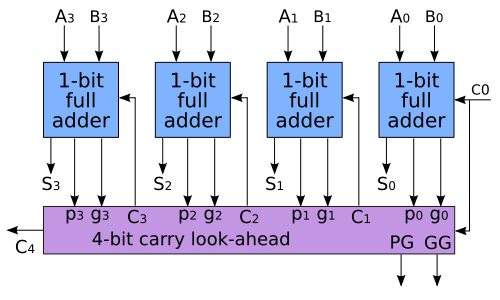
\includegraphics[width=0.75\textwidth]{carry.png}
            \caption{Circuit fabriquant un carry lookahead}
            \label{fig:question}
        \end{figure}
\end{frame}

\begin{frame}{La Clock}
    fonctionnement clock
\end{frame}
    
\begin{frame}
\frametitle{Conclusion}
\begin{itemize}
    \item sysnum c a chier
    \item iris c une grosse pute
\end{itemize}
\end{frame}

\end{document}
